\documentclass[a4paper, 11pt]{article}
\usepackage[utf8]{inputenc}
\usepackage{float}
\usepackage{graphicx}
\usepackage{url}
\usepackage{enumitem}
\usepackage{subcaption}

\setlist[itemize]{itemsep=0.5pt, parsep=0.5pt, topsep=0pt, partopsep=0pt}
\setlist[enumerate]{itemsep=0.5pt, parsep=0.5pt, topsep=0pt, partopsep=0pt}

%opening
\title{HW2 Report, Rudy: A Small Routing Protocol}
\author{David Fischer}
\date{\today{}}

\begin{document}

\maketitle

\section{Introduction}

\textit{Summary of the work you've done, what are the topics we cover
  in this seminar, etc. Remember that you should deliver this report
  at the start of the seminar.}

What is the main topic related to distributed systems covered in this seminar?
Why is it important?

\section{Main problems and solutions}

\subsection{Module Based Approach}

% trouble starting out & seeing bigger picture/correlation
% solved by: writing test functions based on report contents

\subsection{Debugging Final Implementation}

% logging difficulties, router processes dilluting log output
% solved by cleaning up logging

\subsection{Duplicate Updates and Broadcasts}

% biggest troubling issue I couldn't get to the bottom of, because it didn't really matter for testing (2 updates sufficed)
% solved by manually stepping through the code and adding logging at the critical sections

\textit{Summarize your problems, proposed solutions, etc. You do not
  need to copy\&paste your code. Only if needed, you may write down
  small code snipeds to show how you have solved a specific
  problem/question.}

Did you find any specific problem with the development of your
solution?  How did you solve it?

\begin{verbatim}
this(X) ->
    Y = is(X),
    a(test(Y)).
\end{verbatim}

\section{Evaluation}

To efficiently evaluate and debug the implementation, a testing module to set up multiple nodes, their connections, and messaging across different countries (machines) was created.
Figure \ref{fig:map1} shows the complete testing environment.

\begin{figure}[H]
  \begin{center}
    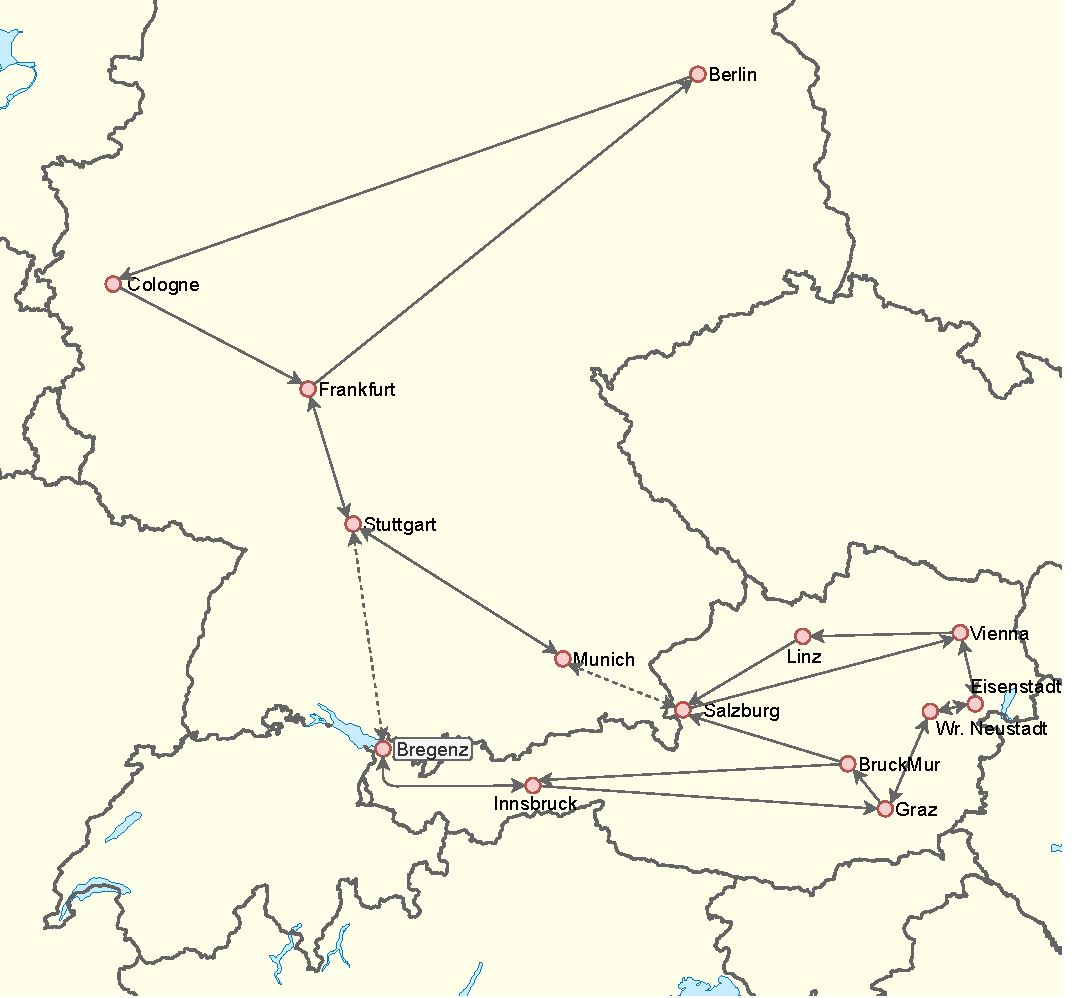
\includegraphics[width=\textwidth]{graphics/map_routy.pdf}
    \caption{Map of routers used for evaluation}
    \label{fig:map1}
  \end{center}
\end{figure}

% removing routers either through deletion or them going down can cause infinite loops between routers

%  1. salzburg goes down
% 2. vienna detects the 'DOWN' message and removes salzburg from its routing table
% 3. But linz still thinks salzburg exists and has a route to vienna through salzburg
% 4. When you send a message to vienna:
%   - linz routes it to salzburg (which is dead)
%   - The message bounces back or gets lost
%   - Or worse, if there are backup paths, it creates routing loops


\section{Conclusions}

% many of the functions aren't implemented as functional, you can tell the object oriented background

% future development: automatically/periodically update & broadcast like OSPF, proper logging, reducing the size of the router function in the routy module

What have you learnt from the problem presented?
Was it useful?

\end{document}
